\clearpage
\newpage
\section*{Extended Data}
\pagebreak

\renewcommand{\figurename}{Extended Data Fig.}
\renewcommand{\tablename}{Extended Data Table}
% \renewcommand{\thetable}{S\arabic{table}}
\setcounter{figure}{0}

\begin{figure}[t]
\centering
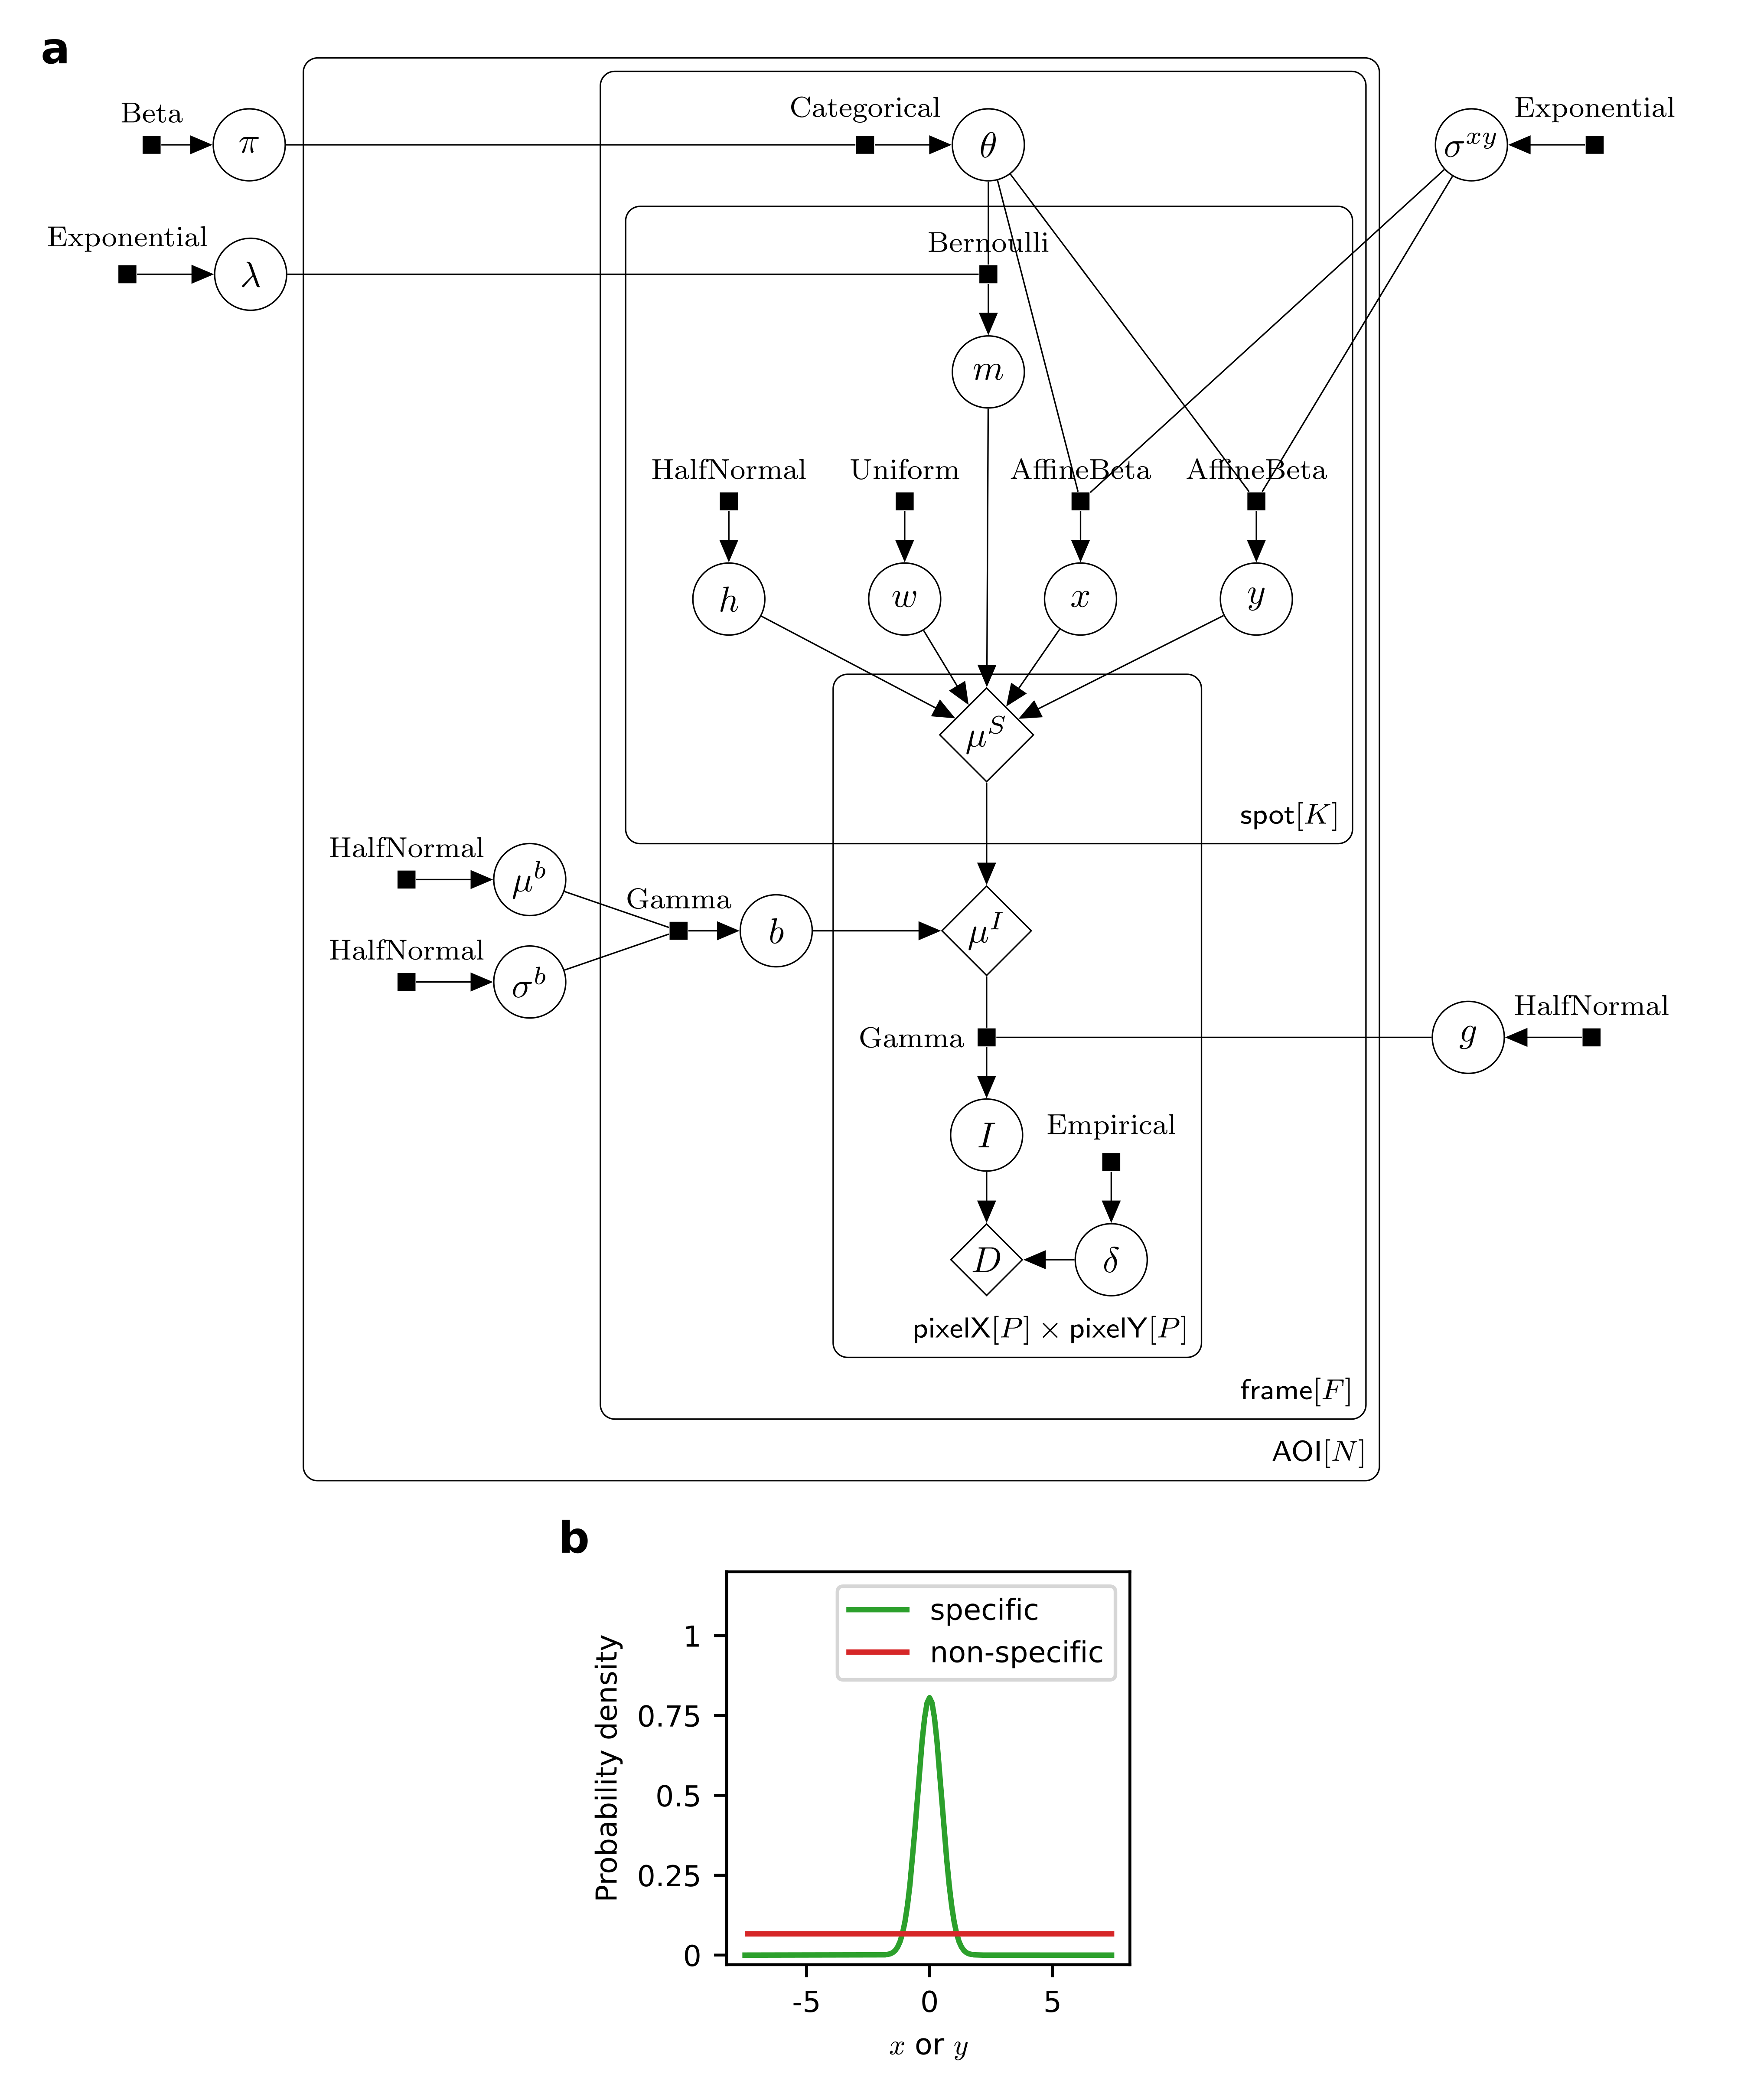
\includegraphics[width=183mm]{extended-data/figure1/figure1.png}
\label{fig:full_model}
\end{figure}

%\addtocounter{figure}{-1}
\begin{figure} [t]
\caption{\textbf{Extended graphical representation of the generative probabilistic model and the prior distributions for $x$ and $y$ spot position parameters.} \textbf{a}, Directed factor graph representation (ref) of model parameters and parameter distributions. Model parameters are depicted as circles, parameter distributions as small filled squares, and deterministic functions as diamonds. Names of the probability distributions are written next to the squares. Input parameters and output parameters are connected by lines, with an arrow pointing towards the dependent parameter. Observed image ($D$) is the sum of the noisy photon-dependent image ($I$) and the photon-independent camera offset ($\delta$). The dashed box represents selection of spot parameters based on the spot existence indicator $m$. Plates (rounded rectangles) contain nodes that are repeated for the number of instances displayed at the bottom-right corner: number of AOIs ($N$), frame count ($F$), maximum number of spots in a single image ($K=2$), and number of image pixels ($P \times P$). \textbf{b}, Prior distributions of $x$ and $y$ for specific and non-specific binding. Probability densities for $x$ and $y$ are defined in the range of the image $-(P+1)/2$, $(P+1)/2$ and are conditional on the identity of the spot (specific or non-specific).  Probability densities for $x$ and $y$ parameters are identical. }
\end{figure}
\clearpage

\begin{figure}[h]
\centering
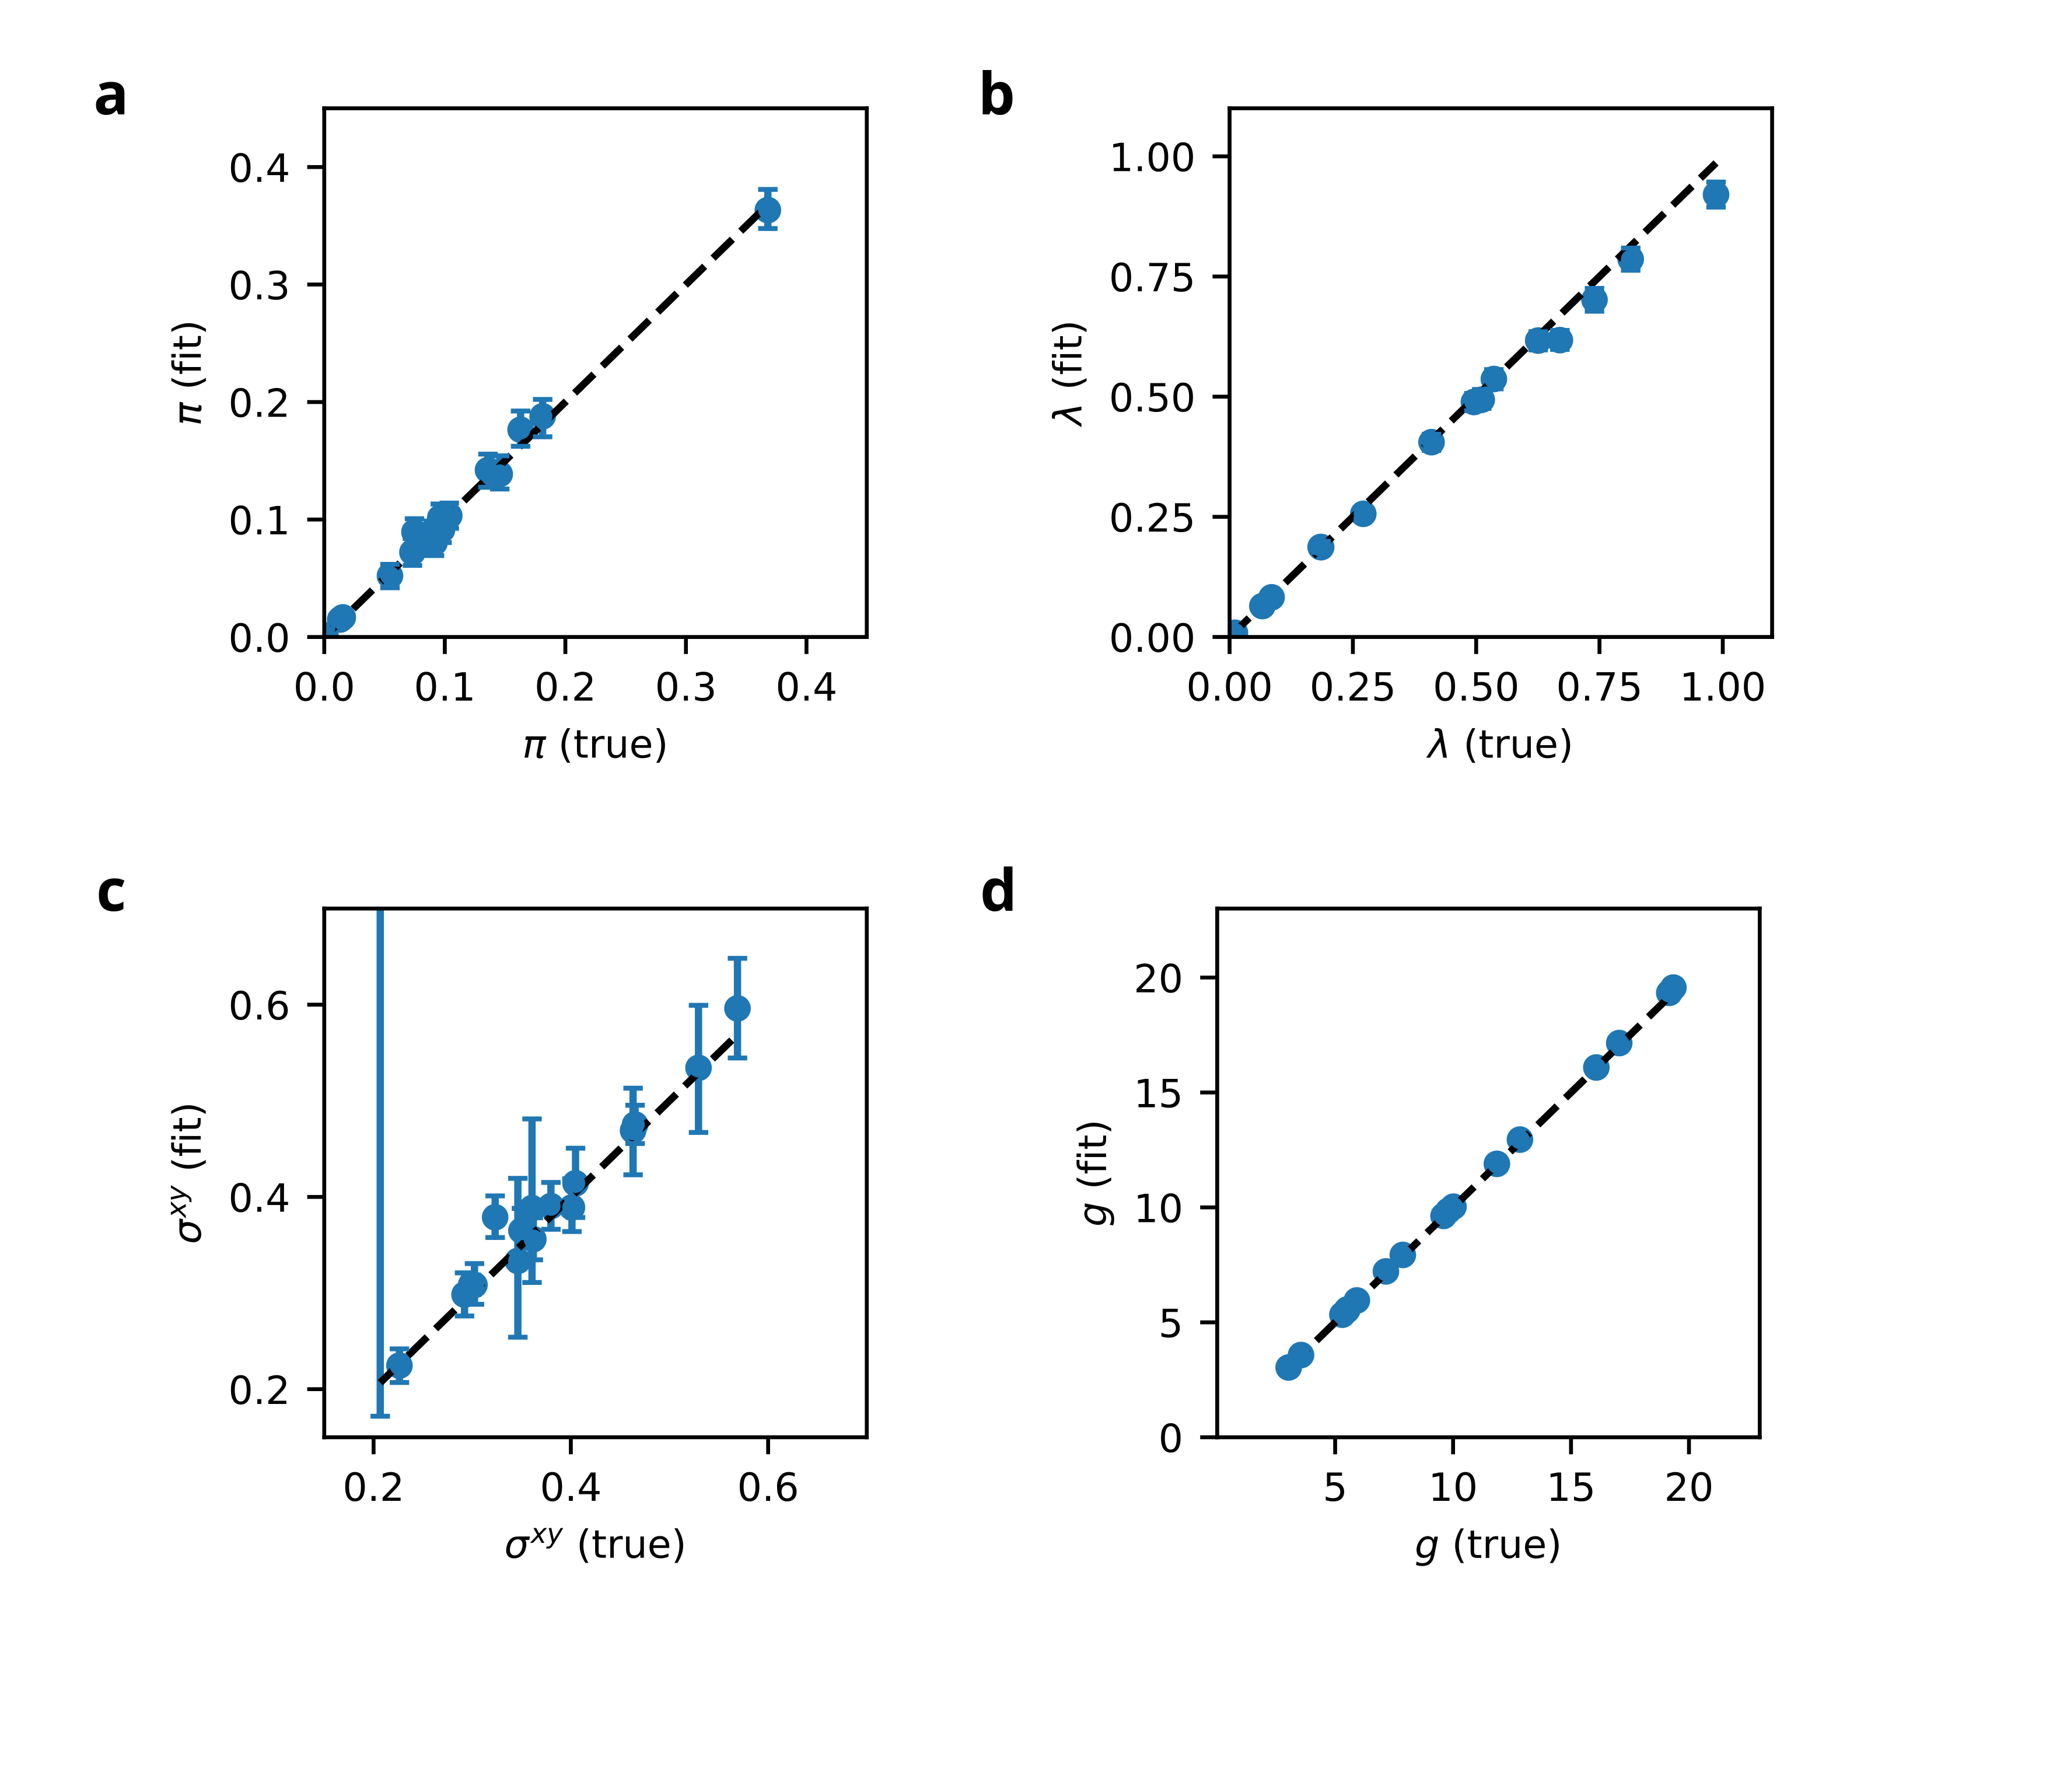
\includegraphics[width=150mm]{extended-data/figure2/figure2.png}
\caption{\textbf{Tapqir analysis of image data simulated using a broad range of global parameters.} Simulations (see Methods) consist of 17 datasets where global parameters ($\pi$, $\lambda$, $\sigma^{xy}$, and $g$) where randomly generated for each dataset (Supplementary Data 2). Simulated data were fit with Tapqir, and parameter values from the fit are plotted against the true parameter values (circles). To guide the eye, dashed lines  indicate identical true and fit values. \textbf{a}, Average specific binding probability $\pi$. \textbf{b}, Nonspecific binding rate $\lambda$. \textbf{c}, Proximity parameter $\sigma^{xy}$. \textbf{d}, Gain of the camera $g$. }
\label{fig:tapqir_global}
\end{figure}
\pagebreak

\begin{figure}[t]
\centering
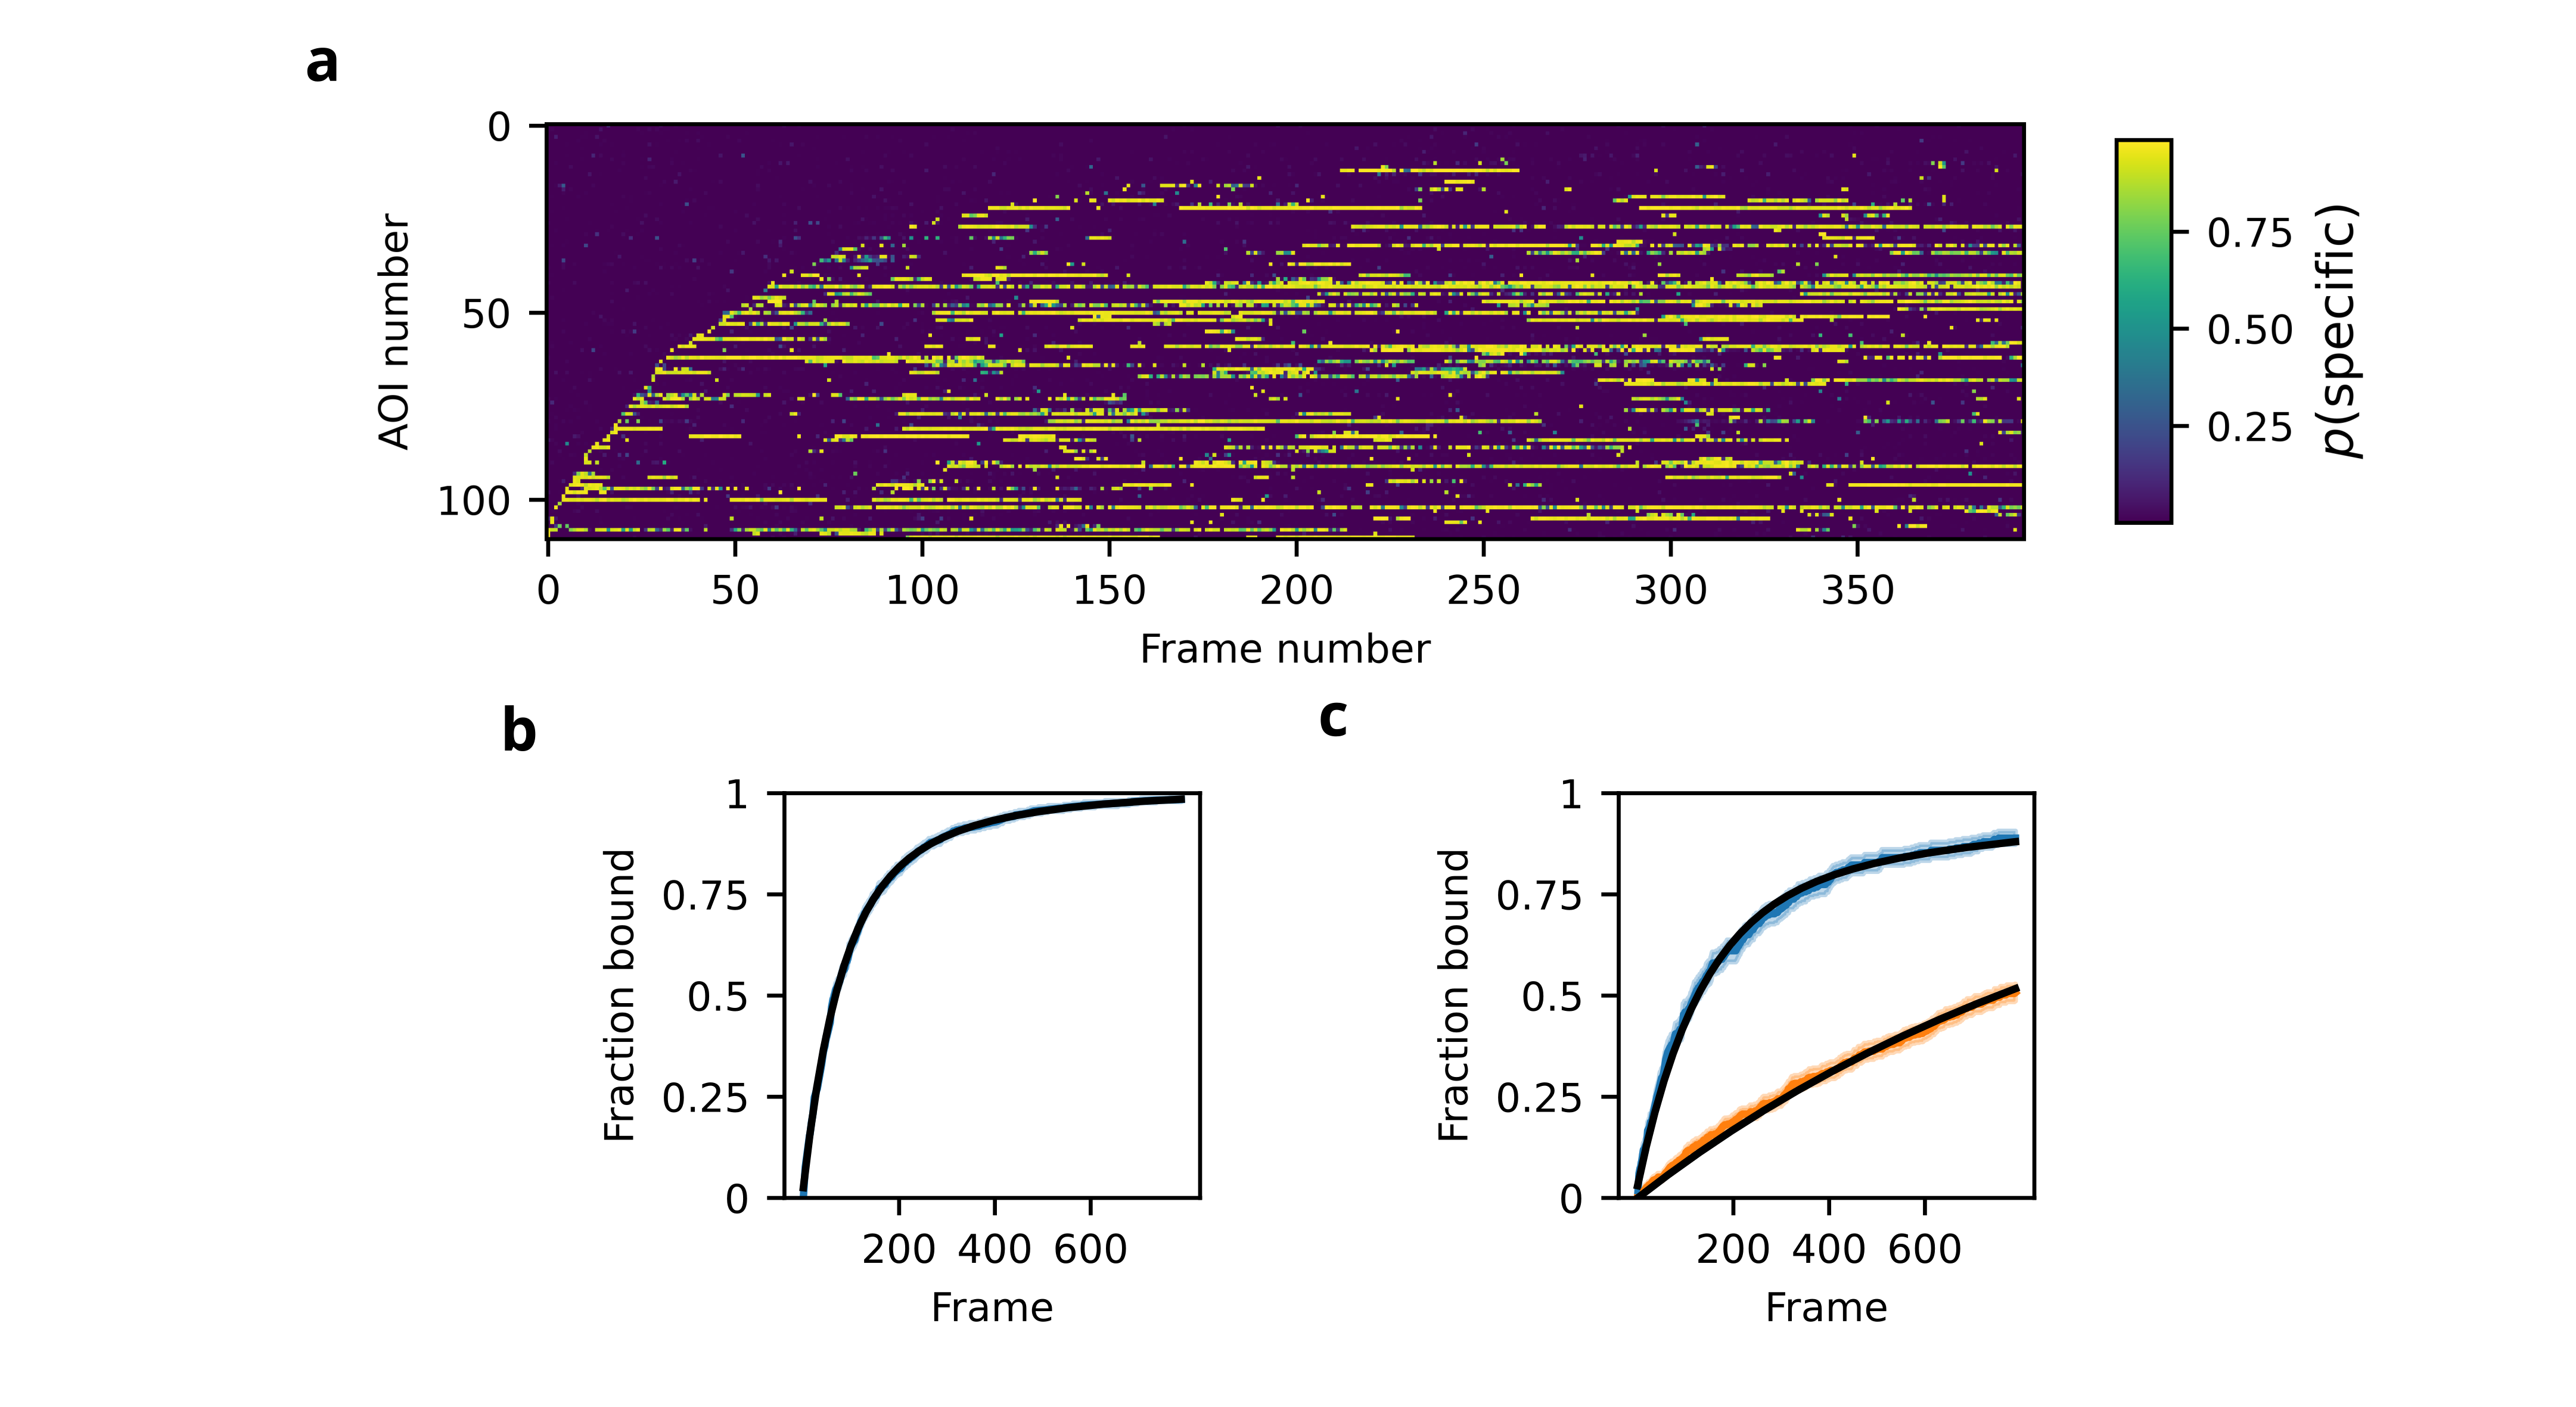
\includegraphics[width=\textwidth]{extended-data/figure3/figure3.png}
\caption{\textbf{Time-to-first binding analysis of experimental data.}  Determining association rates for experimental CoSMoS data using the time-to first binding analysis. \textbf{a}, Rastergram representation of $p(\mathsf{specific})$ (color scale) for every 3\textsuperscript{rd} AOI and every 2\textsuperscript{nd} frame of Rbp1\textsuperscript{SNAP549}-DNA\textsuperscript{488} dataset (Extended Data Table 1). DNA locations ordered by time-to-first binding. \textbf{b,c}, Determining the association rate constant for the same data set by  time-to-first-binding analysis using Tapqir (\textbf{b}: $k_\mathrm{a} = (3.5\pm0.4) \times 10^{-3}$ s$^{-1}$, $k_\mathrm{ns} = (1.27\pm0.27) \times 10^{-3}$ s$^{-1}$) and an empirical spot-picker method (\textbf{c}: $k_\mathrm{a} = (2.2\pm0.2) \times 10^{-3}$ s$^{-1}$, $k_\mathrm{ns} = (3.1\pm0.2) \times 10^{-4}$ s$^{-1}$) (ref).   Cumulative fraction of target sites that exhibited one or more binding events by the indicated time (blue) and fit curve (black) yielding best-fit values for $k_\mathrm{a}$, $k_\mathrm{ns}$, and $A_\mathrm{f}$. Shading indicates 68\% confidence interval.
}
\label{fig:rpb1snap549}
\end{figure}
\pagebreak
% \textbf{a}, Rastergram representation of Tapqir-calculated target-specific spot  probabilities $p(\mathsf{specific})$ (color scale) for every 13\textsuperscript{th} frame of data at 102 different target locations.  AOIs were ordered by decreasing times-to-first-binding. Data set: $\sigma^{54}$RNAPCy3-597P255 in Extended Data Table 1. \textbf{b,c}, Determining the association rate constant for the same data set by  time-to-first-binding analysis using Tapqir (\textbf{b}: $k_\mathrm{a} = (6.74\pm0.43) \times 10^{-3}$ s$^{-1}$, $k_\mathrm{ns} = (5.8\pm1.7) \times 10^{-4}$ s$^{-1}$) and an empirical spot-picker method (\textbf{c}: $k_\mathrm{a} = (4.8\pm0.6) \times 10^{-3}$ s$^{-1}$, $k_\mathrm{ns} = (5.4\pm1.0) \times 10^{-5}$ s$^{-1}$) (ref).   Cumulative fraction of target sites that exhibited one or more binding events by the indicated time (blue) and fit curve (black) yielding best-fit values for $k_\mathrm{a}$, $k_\mathrm{ns}$, and $A_\mathrm{f}$. Shading indicates 68\% confidence interval. Fitting protocol is different for the two methods; the spot-picker method fits both the target sites and off-target control data (orange) whereas Tapqir incorporates the control data in its $p(\mathsf{specific})$ calculation.
\begin{figure}[t]
\centering
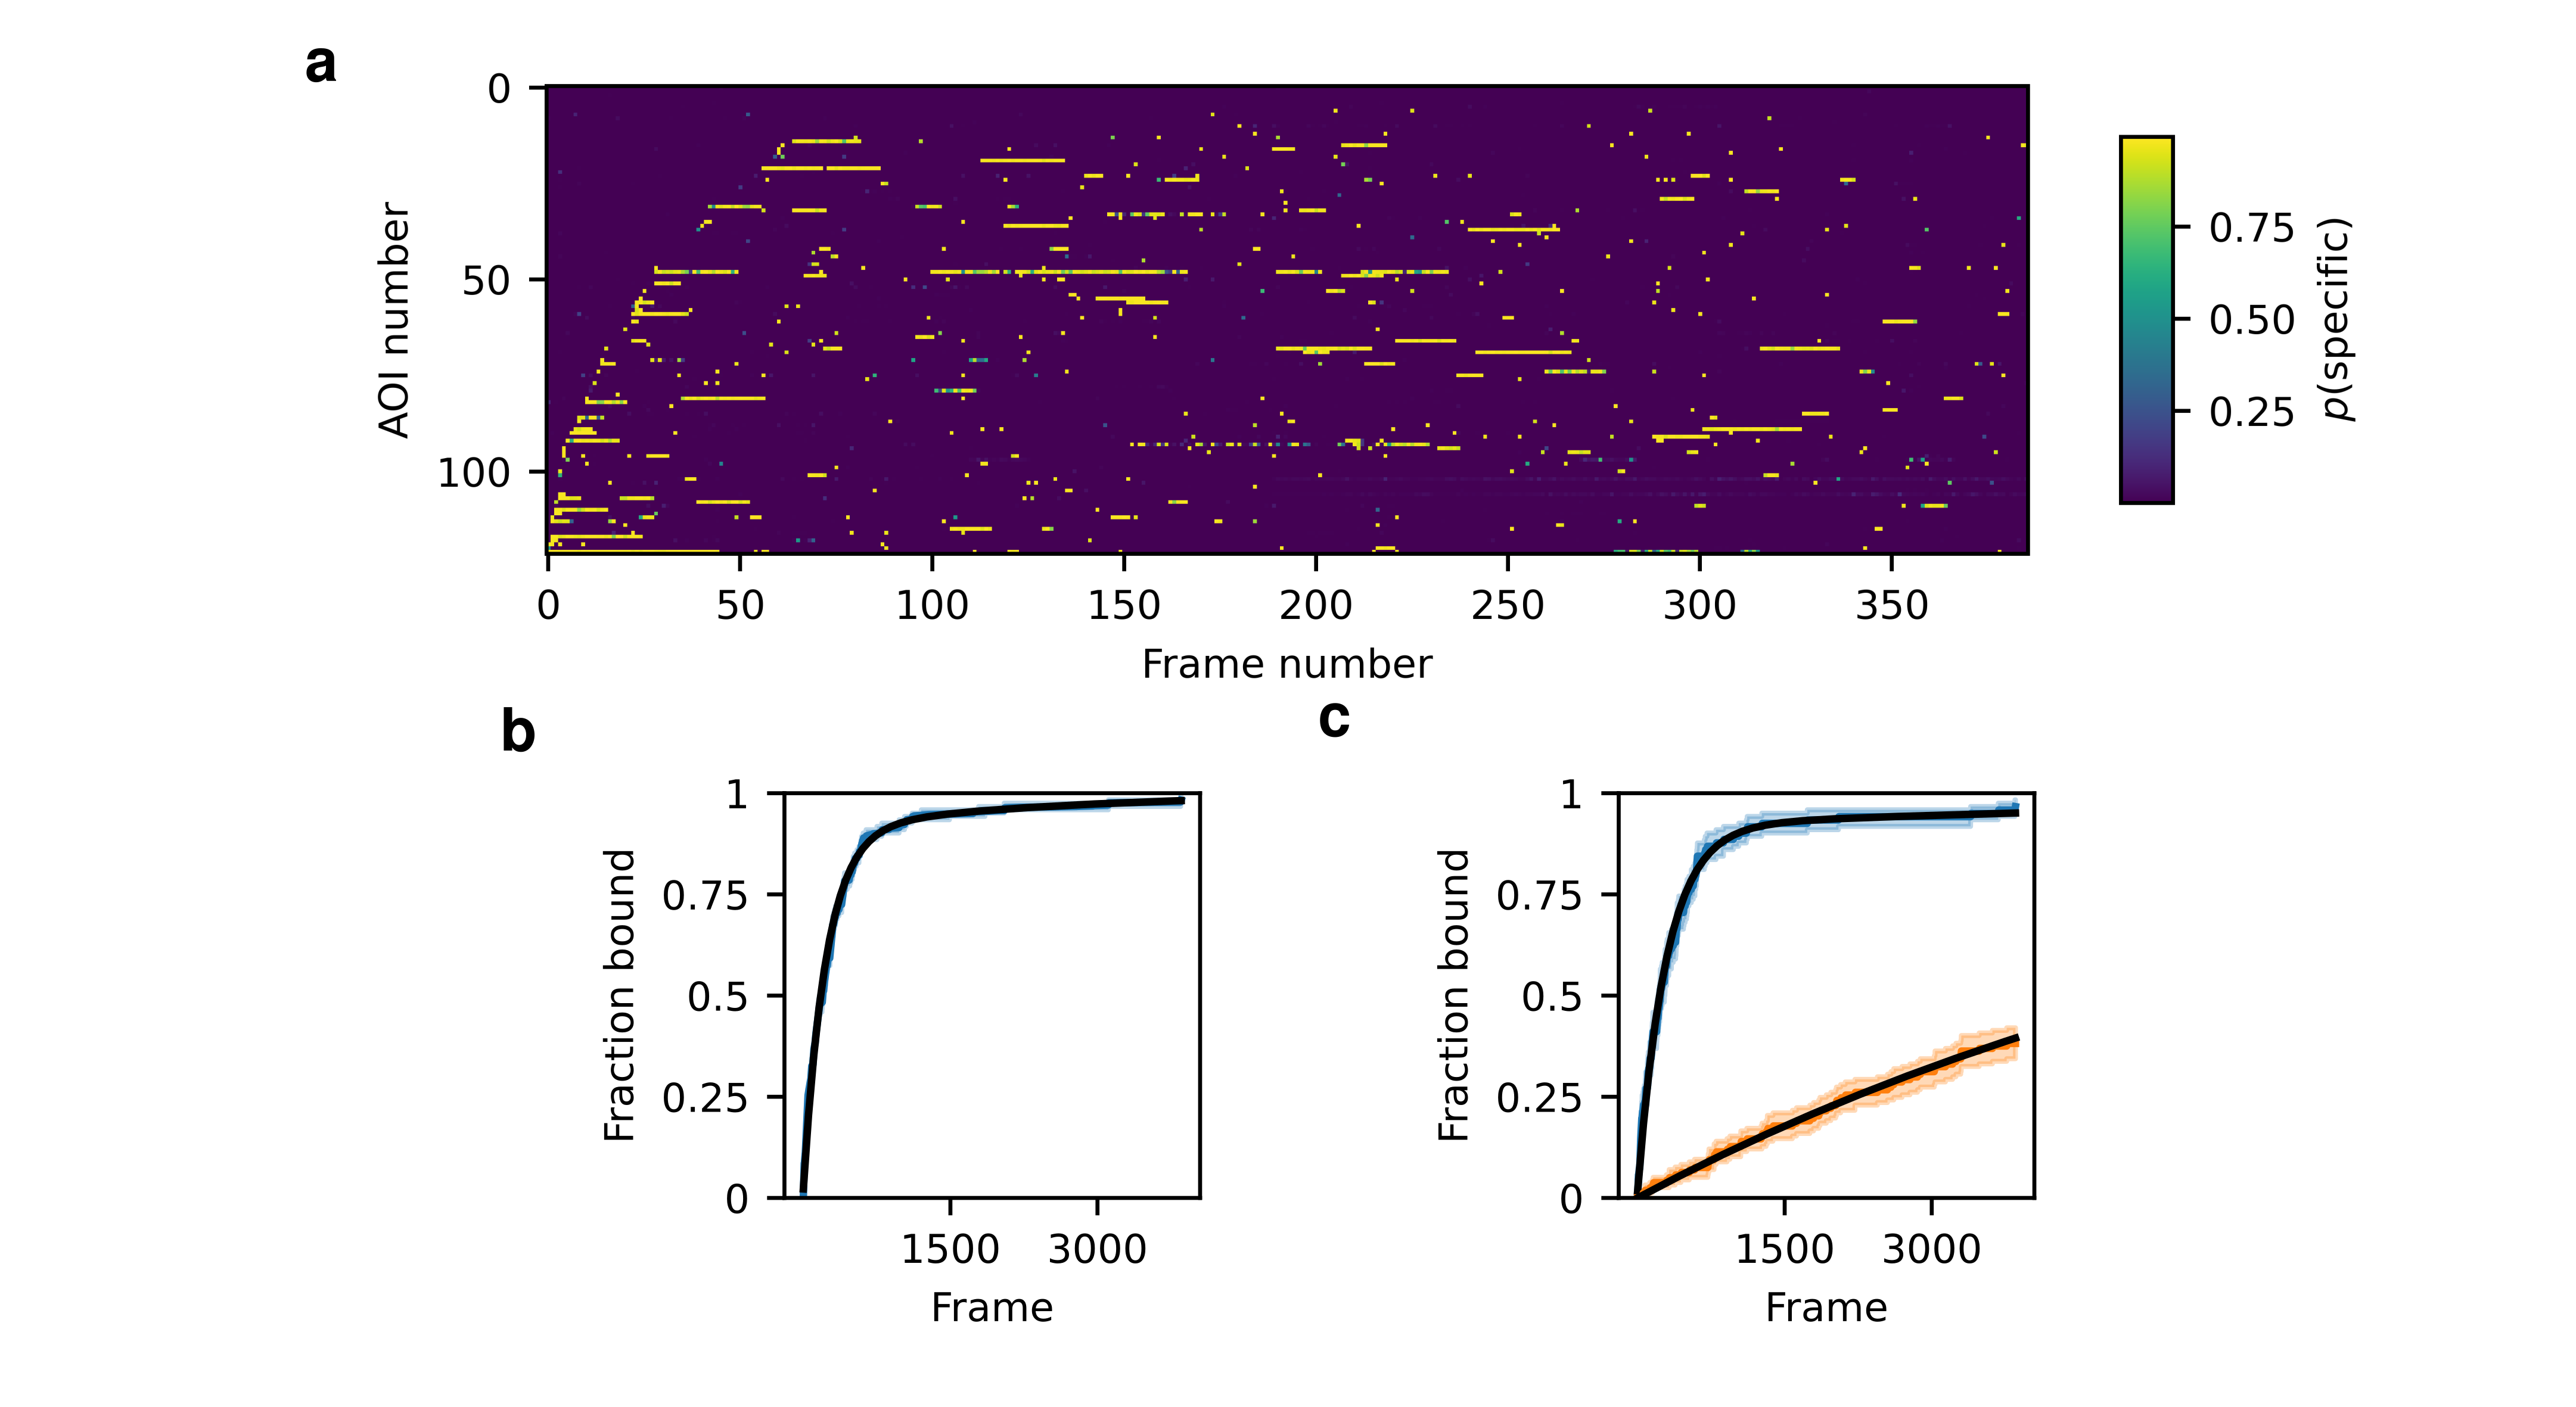
\includegraphics[width=\textwidth]{extended-data/figure4/figure4.png}
\caption{\textbf{Time-to-first binding analysis of experimental data.}  \textbf{a}, Rastergram representation of Tapqir-calculated target-specific spot  probabilities $p(\mathsf{specific})$ (color scale) for every 10\textsuperscript{th} frame of data at 122 different target locations.  AOIs were ordered by decreasing times-to-first-binding. Data set: $\sigma^{54}$RNAPCy3-598P2993 in Extended Data Table 1. \textbf{b,c}, Determining the association rate constant for the same data set by  time-to-first-binding analysis using Tapqir (\textbf{b}: $k_\mathrm{a} = (4.15\pm0.35) \times 10^{-3}$ s$^{-1}$, $k_\mathrm{ns} = (7.1\pm2.5) \times 10^{-4}$ s$^{-1}$) and an empirical spot-picker method (\textbf{c}: $k_\mathrm{a} = (3.2\pm0.3) \times 10^{-3}$ s$^{-1}$, $k_\mathrm{ns} = (1.3\pm0.2) \times 10^{-4}$ s$^{-1}$) (ref). Cumulative fraction of target sites that exhibited one or more binding events by the indicated time (blue) and fit curve (black) yielding best-fit values for $k_\mathrm{a}$, $k_\mathrm{ns}$, and $A_\mathrm{f}$. Shading indicates 68\% confidence interval.
}
\label{fig:sigma54_298P2993}
\end{figure}
\clearpage
\pagebreak

\begin{table}[h]
\caption{\label{tab:datasets} \textbf{Experimental datasets.}}
% Use "S" column identifier to align on decimal point 
\begin{tabular}{lrrrrrr}
\toprule
Dataset & size & SNR & $\pi$ & $\lambda$ & $g$ & $\sigma^{xy}$ \\
\midrule
Rpb1\textsuperscript{SNAP549} & \begin{tabular}[x]{@{}c@{}}$N = 331$, $F = 790$\\$N_c = 526$, $F_c = 526$\end{tabular} & 1.61 &
0.114 & 0.320 & 6.44 & 0.575 \\
\midrule
NusG & \begin{tabular}[x]{@{}c@{}}$N = 122$, $F = 3855$\\$N_c = 157$, $F_c = 3855$\end{tabular} & 4.37 & $0.030$ & $0.0772$ & $16.91$ & $0.384$ \\
\midrule
$\sigma^{54}$ & \begin{tabular}[x]{@{}c@{}}$N = 102$, $F = 4407$\\$N_c = 127$, $F_c = 4407$\end{tabular} & 3.87 & 0.073 & 0.149 & 11.414 & 0.448 \\
\bottomrule
\multicolumn{7}{l}{\footnotesize{\parbox{4.5in}{$^{1}$ Single molecule experiment measuring the binding rate of $\sigma^{54}$RNAP labeled with Cy3 to DNA where the target site for the polymerase on the DNA was bracketed different length (598P255) blue in Fig. 1E in https://www.pnas.org/content/pnas/110/24/9740.full.pdf. $\sigma^{54}$ - 598P2993}}} \\
\end{tabular}
\end{table}
\clearpage
\pagebreak

%\newcommand{\specialcell}[2][c]{%
%  \begin{tabular}[#1]{@{}r@{}}#2\end{tabular}}

% \multicolumn{6}{l}{\footnotesize{\parbox{0.9\textwidth}{$^{1}$For each dataset the first row is the randomized parameter value used in the simulation and the second row gives posterior predictions of parameter values and classification accuracy statistics. Each of the four parameters $\pi$, $\lambda$, $g$, and $\sigma^{xy}$ were independently and randomly selected from a broad range that encompasses typical experimental values. $N = 5$, $F = 500$, $N_c = 5$, $F_c = 500$, $h = 3000$, $w = 1.4$, $b = 150$, $\delta = 90$}}} \\
% \multicolumn{6}{l}{\footnotesize{\parbox{0.9\textwidth}{$^2$See Methods for SNR calculation.}}}



% \multicolumn{10}{l}{\footnotesize{\parbox{4in}{$^1$Parameters $N=5$, $F=500$, $N_c=5$, $F_c=500$, $b=150$, $w=1.4$, $\pi=0.15$, $\lambda=0.15$, $g=7$, $\sigma^{xy}=0.2$, $\delta=150$}}}

\begin{table}[h]
\caption{\label{tab:dist} \textbf{Probability distributions used in the model.}}
\begin{tabular}{l l}
\toprule
Distribution & PDF \\
\midrule
$x \sim \mathbf{AffineBeta}(\mu, \nu, a, b)$ &
    $\dfrac{y^{\alpha-1}(1-y)^{\beta-1}}{\text{B}(\alpha, \beta)}$
    where $\alpha=\dfrac{\nu (\mu-a)}{b-a}$, $\beta=\dfrac{\nu (b-\mu)}{b-a}$, and $y = \dfrac{x-a}{b-a}$ \\
$x \sim \mathbf{Bernoulli}(\pi)$ &
    $\pi^x (1-\pi)^{1-x}$ \\
$x \sim \mathbf{Beta}(\alpha, \beta)$ &
    $\dfrac{x^{\alpha-1}(1-x)^{\beta-1}}{\text{B}(\alpha, \beta)}$ \\
$x \sim \mathbf{Categorical}_{\{z_i\}^k_{i=1}}(\mathbf{p})$ &
    $\prod_{i=1}^k p_i^{[x=z_i]}$ \\
$x \sim \mathbf{Gamma}(\mu, \sigma)$ &
    $\dfrac{\beta^\alpha}{\Gamma(\alpha)}x^{\alpha-1} e^{-\beta x}$
    where $\alpha = \dfrac{\mu^2}{\sigma^2}$ and $\beta = \dfrac{\mu}{\sigma^2}$ \\
$x \sim \mathbf{HalfNormal}(\sigma)$ &
    $\dfrac{\sqrt{2}}{\sigma \sqrt{\pi}} \exp \left( -\dfrac{x^2}{2\sigma^2} \right)$
    for  $x > 0$ \\
$k \sim \mathbf{TruncatedPoisson}(\lambda, K) $ & $ \begin{cases} 1 - e^{-\lambda} \sum_{i=0}^{K-1} \dfrac{\lambda^i}{i!} & \textrm{if $k = K$} \\ \dfrac{\lambda^k e^{-\lambda}}{k!} & \textrm{otherwise} \end{cases} $ \\
$x \sim \mathbf{Uniform}(a, b)$ &
    $\dfrac{1}{b-a}$ for $x \in [a, b]$ \\
\bottomrule
\end{tabular}
\end{table}